\section{Verificação e validação}
\subsection{Métodos de verificação}

\begin{frame}{Vulnerabilidades em CIs}
    \begin{block}{}
    Grande parte das vulnerabilidades encontradas em CIs escritos em Solidity poderiam ter sido evitadas com a ajuda de \textbf{análise formal} e \textbf{verificação} desses contratos antes de serem implantados na blockchain.
    \end{block}
    \begin{itemize}
        \item Linguagens como Solidity não foram desenvolvidas para serem verificadas formalmente;
        \item Solidity não é uma linguagem perfeita;
        \item Questões relacionadas com a execução dos CIs na Ethereum muitas vezes não são compreendidas pelos desenvolvedores.
    \end{itemize}
\end{frame}

\begin{frame}{Vulnerabilidades em CIs - Como evitar?}
    \textbf{Serviços de auditoria:}
    \begin{itemize}
        \item Organizações: OpenZeppeling, Solidified e SmartDec;
        \item Podem ser muito custosos para pequenas organizações e desenvolvedores autônomos.
    \end{itemize}
    \begin{exampleblock}{\textbf{Solução}}
    \textbf{Frameworks e ferramentas de verificação de CIs}
    \end{exampleblock}
\end{frame}

\begin{frame}{Verificação de CIs - Frameworks e ferramentas}
    Dois tipos de verificação:
    \begin{itemize}
        \item Proativa:
        \begin{itemize}
            \item Aplicada antes da implantação.
        \end{itemize}
        \item Reativa:
        \begin{itemize}
            \item Monitoramento do contrato durante a execução;
            \item Verificação em \textbf{tempo de execução}.
        \end{itemize}
    \end{itemize}
\end{frame}

\begin{frame}{Verificação de CIs - Frameworks e ferramentas}
	Métodos de verificação:
	\begin{itemize}
		\item Análise de código:
		\begin{itemize}
			\item Pode ser \textbf{estática}, \textbf{dinâmica} ou \textbf{híbrida};
			\item \textbf{Execução simbólica}.
		\end{itemize}
		\item Métodos formais:
		\begin{itemize}
			\item \textit{Model checking};
			\item Demonstração de teoremas;
			\item Verificação dedutiva.
		\end{itemize}		
	\end{itemize}
\end{frame}

\begin{frame}{Análise de código}
	\begin{itemize}
		\item Estratégia geralmente automatizada;
		\item Detecção de erros;
		\item Identificação de vulnerabilidades;
		\item Aspectos analisados:
		\begin{itemize}
			\item Fluxo de controle;
			\item Fluxo de dados;
			\item Interface;
			\item Fluxo de informações;
			\item Caminhos de execução.
		\end{itemize}
		\item Verificação pode ser \textbf{estática}, \textbf{dinâmica} ou \textbf{híbrida};
		\item Normalmente é utilizada alguma representação intermediária estruturada:
		\begin{itemize}
			\item Grafo de fluxo de controle;
			\item Árvore sintática em XML.
		\end{itemize}
		\item \textbf{Execução simbólica}.
	\end{itemize}
\end{frame}

\begin{frame}{\textit{Model checking}}
	\begin{itemize}
		\item Verificação de sistemas de transição de estados;
		\item Três etapas:
		\begin{itemize}
			\item Modelagem;
			\item Especificação: especificação formal dos requisitos;
			\begin{itemize}
				\item Propriedades: Lógicas temporais.
			\end{itemize}
			\item Verificação.
		\end{itemize}
	\end{itemize}
	\begin{figure}[!htb]
		\centering
		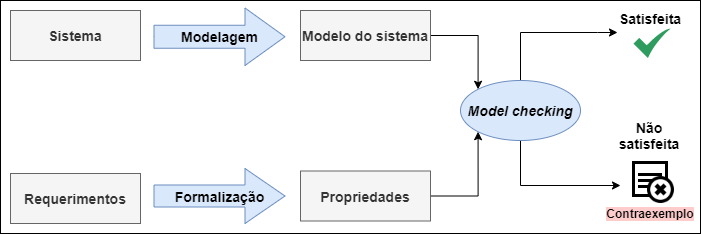
\includegraphics[scale=0.4]{figuras/verificacao/model-checking.png}
	\end{figure}    
\end{frame}

\begin{frame}{Verificação de CIs - Frameworks e ferramentas}
	Métodos de verificação:
	\begin{itemize}		
		\item \textit{Fuzzing}:
		\begin{itemize}
			\item Geração de mutações.
		\end{itemize}
		\item Técnicas de Inteligência Artificial (IA):
		\begin{itemize}
			\item \textit{Machine learning} e \textit{deep learning}.
		\end{itemize}
		\item Em tempo de execução:
		\begin{itemize}
			\item Instrumentalização de código.
		\end{itemize}
	\end{itemize}
\end{frame}

